\documentclass[14pt,a4paper]{report}  %紙張設定
\usepackage{xeCJK}%中文字體模組
\setCJKmainfont{標楷體} %設定中文字體
%\setCJKmainfont{MoeStandardKai.ttf}
\newfontfamily\sectionef{Times New Roman}%設定英文字體
%\newfontfamily\sectionef{Nimbus Roman}
\usepackage{enumerate}
\usepackage{amsmath,amssymb}%數學公式、符號
\usepackage{amsfonts} %數學簍空的英文字
\usepackage{graphicx, subfigure}%圖形
\usepackage{fontawesome5} %引用icon
\usepackage{type1cm} %調整字體絕對大小
\usepackage{textpos} %設定文字絕對位置
\usepackage[top=2.5truecm,bottom=2.5truecm,
left=3truecm,right=2.5truecm]{geometry}
\usepackage{titlesec} %目錄標題設定模組
\usepackage{titletoc} %目錄內容設定模組
\usepackage{textcomp} %表格設定模組
\usepackage{multirow} %合併行
%\usepackage{multicol} %合併欄
\usepackage{CJK} %中文模組
\usepackage{CJKnumb} %中文數字模組
\usepackage{wallpaper} %浮水印
\usepackage{listings} %引用程式碼
\usepackage{hyperref} %引用url連結
\usepackage{setspace}
\usepackage{lscape}%設定橫式
\lstset{language=Python, %設定語言
		basicstyle=\fontsize{10pt}{2pt}\selectfont, %設定程式內文字體大小
		frame=lines,	%設定程式框架為線
}
%\usepackage{subcaption}%副圖標
\graphicspath{{./../images/}} %圖片預設讀取路徑
\usepackage{indentfirst} %設定開頭縮排模組
\renewcommand{\figurename}{\Large 圖.} %更改圖片標題名稱
\renewcommand{\tablename}{\Large 表.}
\renewcommand{\lstlistingname}{\Large 程式.} %設定程式標示名稱
\hoffset=-5mm %調整左右邊界
\voffset=-8mm %調整上下邊界
\setlength{\parindent}{3em}%設定首行行距縮排
\usepackage{appendix} %附錄
\usepackage{diagbox}%引用表格
\usepackage{multirow}%表格置中
%\usepackage{number line}
%=------------------更改標題內容----------------------=%
\titleformat{\chapter}[hang]{\center\sectionef\fontsize{20pt}{1pt}\bfseries}{\LARGE 第\CJKnumber{\thechapter}章}{1em}{}[]
\titleformat{\section}[hang]{\sectionef\fontsize{18pt}{2.5pt}\bfseries}{{\thesection}}{0.5em}{}[]
\titleformat{\subsection}[hang]{\sectionef\fontsize{18pt}{2.5pt}\bfseries}{{\thesubsection}}{1em}{}[]
%=------------------更改目錄內容-----------------------=%
\titlecontents{chapter}[11mm]{}{\sectionef\fontsize{18pt}{2.5pt}\bfseries\makebox[3.5em][l]
{第\CJKnumber{\thecontentslabel}章}}{}{\titlerule*[0.7pc]{.}\contentspage}
\titlecontents{section}[18mm]{}{\sectionef\LARGE\makebox[1.5em][l]
{\thecontentslabel}}{}{\titlerule*[0.7pc]{.}\contentspage}
\titlecontents{subsection}[4em]{}{\sectionef\Large\makebox[2.5em][l]{{\thecontentslabel}}}{}{\titlerule*[0.7pc]{.}\contentspage}
%=----------------------章節間距----------------------=%
\titlespacing*{\chapter} {0pt}{0pt}{18pt}
\titlespacing*{\section} {0pt}{12pt}{6pt}
\titlespacing*{\subsection} {0pt}{6pt}{6pt}
%=----------------------標題-------------------------=%             
\begin{document} %文件
\sectionef %設定英文字體啟用
\vspace{12em}
\begin{titlepage}%開頭
\begin{center}   %標題  
\makebox[1.5\width][s] %[s] 代表 Stretch the interword space in text across the entire width
{\fontsize{24pt}{2.5pt}國立虎尾科技大學}\\[18pt]
\makebox[1.5\width][s]
{\fontsize{24pt}{2.5pt}機械設計工程系}\\[18pt]
\sectionef\fontsize{24pt}{1em}\selectfont\textbf
{
\vspace{0.5em}
cd2023 2a-pj1ag2分組報告}\\[18pt]
%設定文字盒子 [方框寬度的1.5倍寬][對其方式為文字平均分分布於方框中]\\距離下方18pt
\vspace{1em} %下移
\fontsize{30pt}{1pt}\selectfont\textbf{網際足球機器人}\\
\vspace{1em}
\sectionef\fontsize{30pt}{1em}\selectfont\textbf
{
\vspace{0.5em}
Web-based Football Scene Design}
 \vspace{2em}
%=---------------------參與人員-----------------------=%             
\end{center}
\begin{flushleft}
\begin{LARGE}

\hspace{32mm}\makebox[5cm][s]
{指導教授:\quad 嚴\quad 家\quad 銘\quad 老\quad 師}\\[6pt]
\hspace{32mm}\makebox[5cm][s]
{班\qquad 級:\quad 四\quad 設\quad 二\quad 甲}\\[6pt]
\hspace{32mm}\makebox[5cm][s]
{學\qquad 生:\quad 第\quad 一\quad 位\quad(41023146)}
\\[6pt]
\hspace{32mm}\makebox[5cm][s]
{\hspace{36.5mm}第\quad 二\quad 位\quad(41023148)}\\[6pt]

%設定文字盒子[寬度為5cm][對其方式為文字平均分分布於方框中]空白距離{36.5mm}\空白1em
\end{LARGE}
\end{flushleft}
\vspace{6em}
\fontsize{18pt}{2pt}\selectfont\centerline{\makebox[\width][s]
{中華民國\hspace{3em} 
112 \quad 年\quad 3\quad 月}}
\end{titlepage}
\newpage
%=---------------報告製作核可證明---------------------=%
 {\renewcommand\baselinestretch{1.4}\selectfont %設定以下行距
 {\begin{center}
    {\fontsize{20pt}{2.5pt} {國立虎尾科技大學 \qquad 機械設計工程系}\\[8pt]{分組報告製作合格認可證明}\\
    \hspace*{\fill} \\ %似enter鍵換行
    \par}
     \end{center}}
    {\begin{textblock}{60}(1.85,0.8)
    \noindent \fontsize{15pt}{16pt}\selectfont 分組報告製作修習學生\enspace:\quad
    {\begin{minipage}[t]{10em}\underline{四設二甲\enspace 41023146 第一位}\\ \underline{四設二甲\enspace 41023148\enspace 第二位}\\  %下劃線符號指令
    \end{minipage}}
         \par} %結束指定行距
    {\renewcommand\baselinestretch{1.2}\selectfont %設定以下行距
    {\begin{textblock}{30}(1.8,4)
    \noindent \fontsize{16pt}{16pt}\selectfont 分組報告題目\enspace :網際手足球場景設計
    \hspace*{\fill} \\
    \hspace*{\fill} \\
    \noindent \fontsize{16pt}{16pt}\selectfont 經評量合格,特此證明
    \hspace*{\fill} \\
    \hspace*{\fill} \\
    \noindent \fontsize{16pt}{16pt} \makebox[6em][s]{評審委員}\enspace:\quad
    {\begin{minipage}[t]{6em} \underline{            }\\[16pt] \underline{            }\\[16pt] \underline{            }\\
    \end{minipage}}
    \end{textblock}}
    {\begin{textblock}{10}(1.8,9)
    {\begin{flushleft}
    \fontsize{16pt}{16pt}\selectfont \makebox[6em][s]{指導老師}\enspace:\quad \underline{            }\\[10pt]
    \hspace*{\fill} \\
    \fontsize{16pt}{2.5pt}\selectfont \makebox[12em][s]{中華民國一一二年}\hspace{2pt}
    \fontsize{16pt}{2.5pt}\selectfont\makebox[8em][s]{三月三十一日}
    \end{flushleft}}
    \end{textblock}}
    \end{textblock}}
     \par} %結束指定行距
     \newpage

%=------------------------摘要-----------------------=%
\renewcommand{\baselinestretch}{1.5} %設定行距
\pagenumbering{roman} %設定頁數為羅馬數字
\clearpage  %設定頁數開始編譯
\sectionef
\addcontentsline{toc}{chapter}{摘~~~要} %將摘要加入目錄
\begin{center}
\LARGE\textbf{摘~~要}\\
\end{center}
\begin{flushleft}
\fontsize{14pt}{20pt}\sectionef\hspace{12pt}\quad 本學期採取個人及團體分組來學習,團體實習目標為開發一款能在 web-based CoppeliaSim 場景中雙方或多方對玩的遊戲。pj3 為八人一組,根據自選產品在期限內完成產品開發,在 w16 現場發表八人協同四週後所完成的產品,在 w17 各組採 OBS + Teams 以影片發表所完成的協同產品。\\[12pt]
\fontsize{14pt}{20pt}\sectionef\hspace{12pt}\quad  接續 pj2,各組須對雙輪車進行設計改良,以提升行進與對戰效率。採 CAD 進行場景與多輪車零組件設計後,轉入足球場景中以鍵盤 arrow keys 與 wasd 等按鍵進行控制,對雙方每組將有四名輪車球員,且每兩人在同一台電腦上操作,完成後各組須在分組網站中提供所有相關檔案下載連結,且提供線上分組簡報與分組 pdf 報告連結。\\[12pt]	
\fontsize{14pt}{20pt}\sectionef\hspace{12pt}\quad 此專題是雙方利用各四台 BubbleRob 多輪車在一足球場景中進行對戰,雙方球門分別設有感測器。 在規定時間內,每進一球即透過程式重新往球場內隨機發球,接續賽局。模擬場景中還須配置 LED 計分板顯示比賽剩餘時間與比分,還需另外建立以機械轉盤傳動計分系統。在 CoppeliaSim 模擬環境中進行測試運用上的可行性並嘗試透過埠號供使用者觀看。\\
  更多詳細內容可以到 https://mdecd2023.github.io/2a3-pj3ag4 了解。\\[10pt]

\end{flushleft}
\newpage
%=--------------------Abstract----------------------=%
\renewcommand{\baselinestretch}{1.5} %設定行距
\addcontentsline{toc}{chapter}{Abstract} %將摘要加入目錄
\begin{center}
\LARGE\textbf\sectionef{Abstract}\\
\begin{flushleft}
\fontsize{14pt}{16pt}\sectionef\hspace{12pt}\quad This semester adopts both individual and group learning approaches. The group project involves developing a web-based game that allows two or more players to interact in a CoppeliaSim simulation environment. For Project 3 (pj3), the group consists of eight members who will collaborate to develop a product of their choice within a given deadline. In Week 16, the group will present the product they have developed over four weeks of collaboration. In Week 17, each group will use OBS + Teams to present their collaborative product through a video presentation.\\[12pt]
\fontsize{14pt}{16pt}\sectionef\hspace{12pt}\quad Continuing from pj2, each group is required to design improvements for a two-wheeled vehicle to enhance its mobility and combat efficiency. Using CAD software, the groups will design the scene and components of the multi-wheel vehicle. The project will then transition to a soccer field scenario, where the vehicle will be controlled using keyboard arrow keys and WASD keys. Each group will have four vehicle players, with two players operating on the same computer. Upon completion, each group must provide download links for all relevant files on the group's website, as well as links to online group presentations and a PDF report.\\[12pt]
\fontsize{14pt}{16pt}\sectionef\hspace{12pt}\quad This project involves a two-player battle using four BubbleRob multi-wheel vehicles in a soccer field scenario. Each player has their own goal equipped with sensors. Within a specified time frame, each goal scored triggers the program to reset and randomly kick off a new ball into the field, continuing the game. The simulation scene also includes an LED scoreboard to display the remaining time and score of the match. Additionally, a mechanical turntable-driven scoring system needs to be created. Feasibility testing and user observation will be conducted in the CoppeliaSim simulation environment, with the option for users to observe through port numbers.\\[12pt]
\end{flushleft}

\newpage
%=------------------------誌謝----------------------=%
\addcontentsline{toc}{chapter}{誌謝}
\centerline\LARGE\textbf{誌謝}\\
\begin{flushleft}
\fontsize{14pt}{2.5pt}\hspace{12pt}\quad 在此鄭重感謝製作以及協助本分組報告完成的所有人員,首先感謝學長範本,讓我們比較好改,也感謝老師平日的教導。
\end{flushleft}
\newpage
%=------------------------目錄----------------------=%
\renewcommand{\contentsname}{\centerline{\fontsize{18pt}{\baselineskip}\selectfont\textbf{目\quad 錄}}}
\tableofcontents  %目錄產生
\newpage
%=-------------------------內容----------------------=%
\chapter{前言}
\renewcommand{\baselinestretch}{10.0} %設定行距
\pagenumbering{arabic} %設定頁號阿拉伯數字
\setcounter{page}{1}  %設定頁數
\fontsize{14pt}{2.5pt}\sectionef
\section{研究動機}
機器學習與各領域結合的應用越來越廣泛,在機電系統採用強化學習是為了讓機電系統的控制達到最佳化。本專題以實體的足球機之機電系統作為訓練模型,將實體機器轉移到虛擬環境進行模擬,為了找到適合的訓練參數,因此將模型簡化後再進行測試各種參數的優劣,透過不斷的訓練來得到一個優化過的對打系統,以下是成品圖。\\

\begin{figure}[hbt!]
\begin{center}
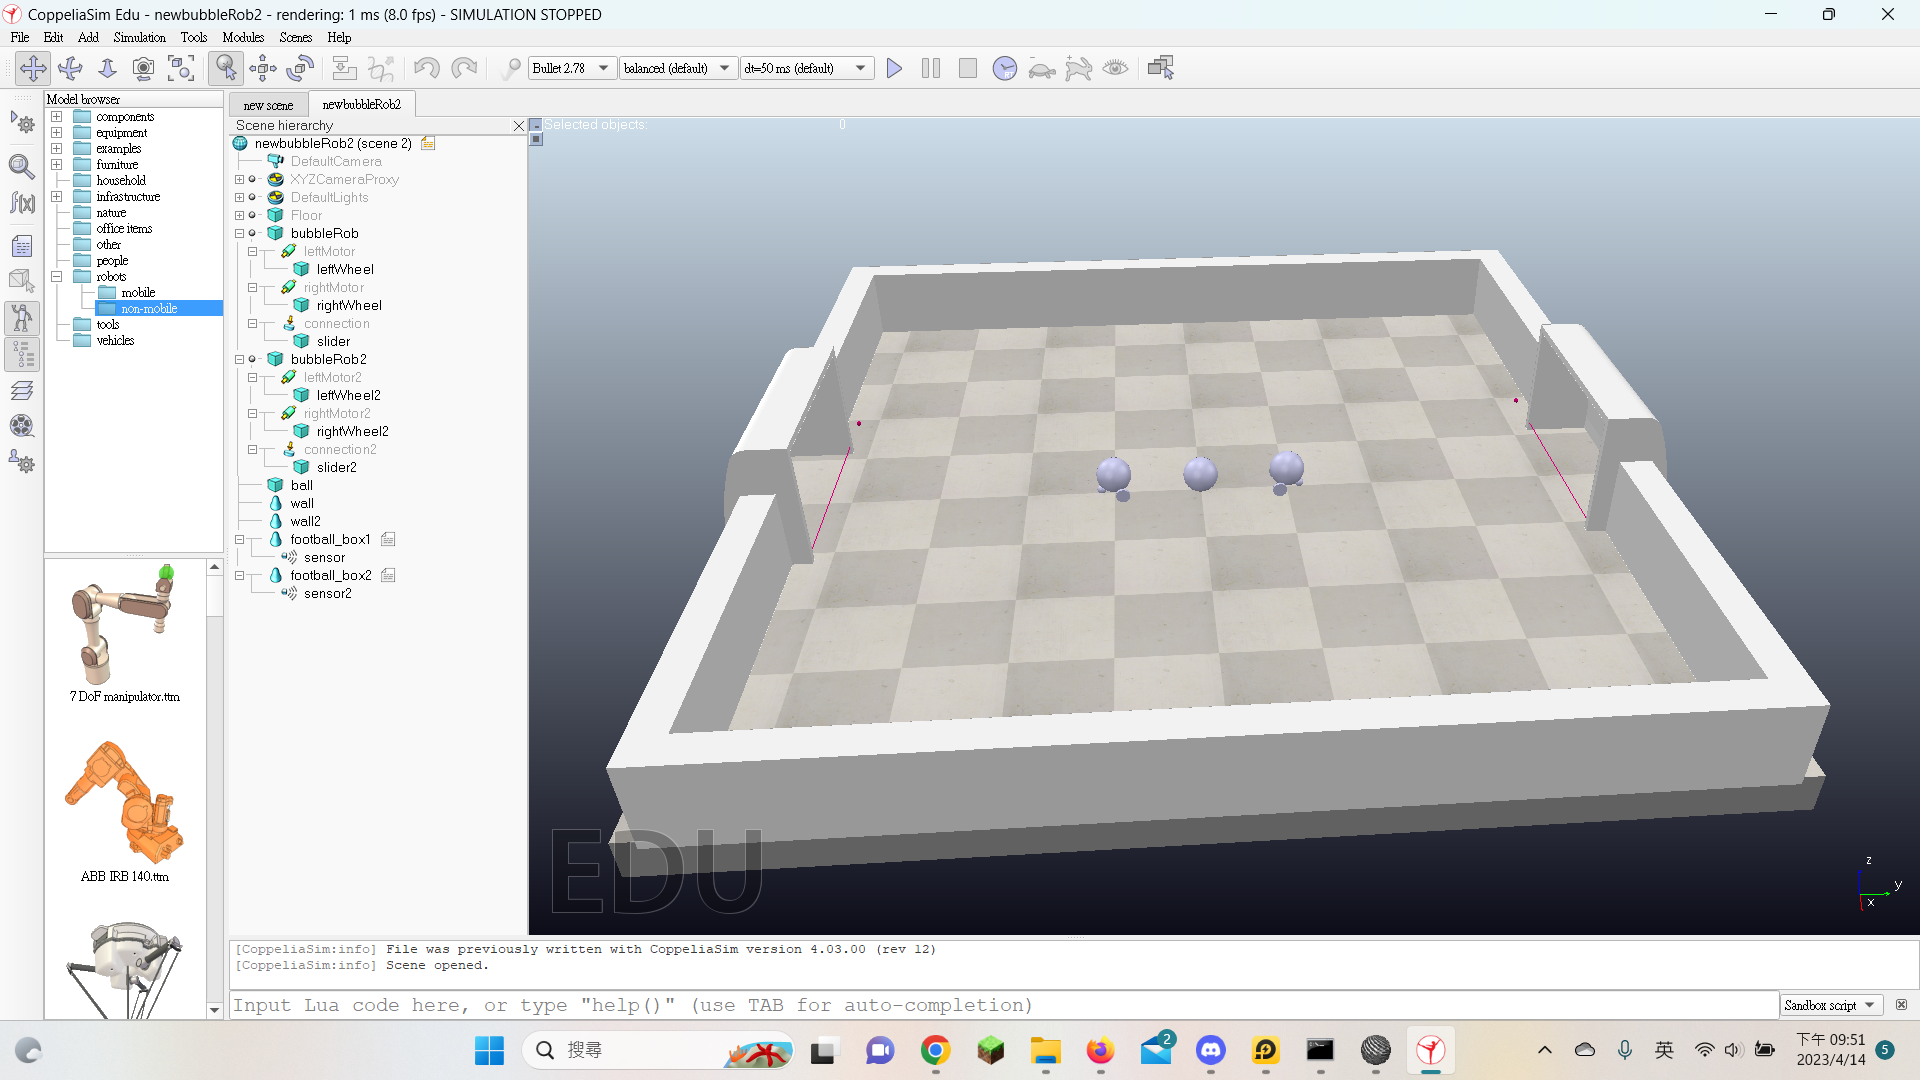
\includegraphics[angle=0,width=17cm]{2023-04-14}
\end{center}
\end{figure}

\newpage
\section{製作過程}
1.首先繪製球框。\
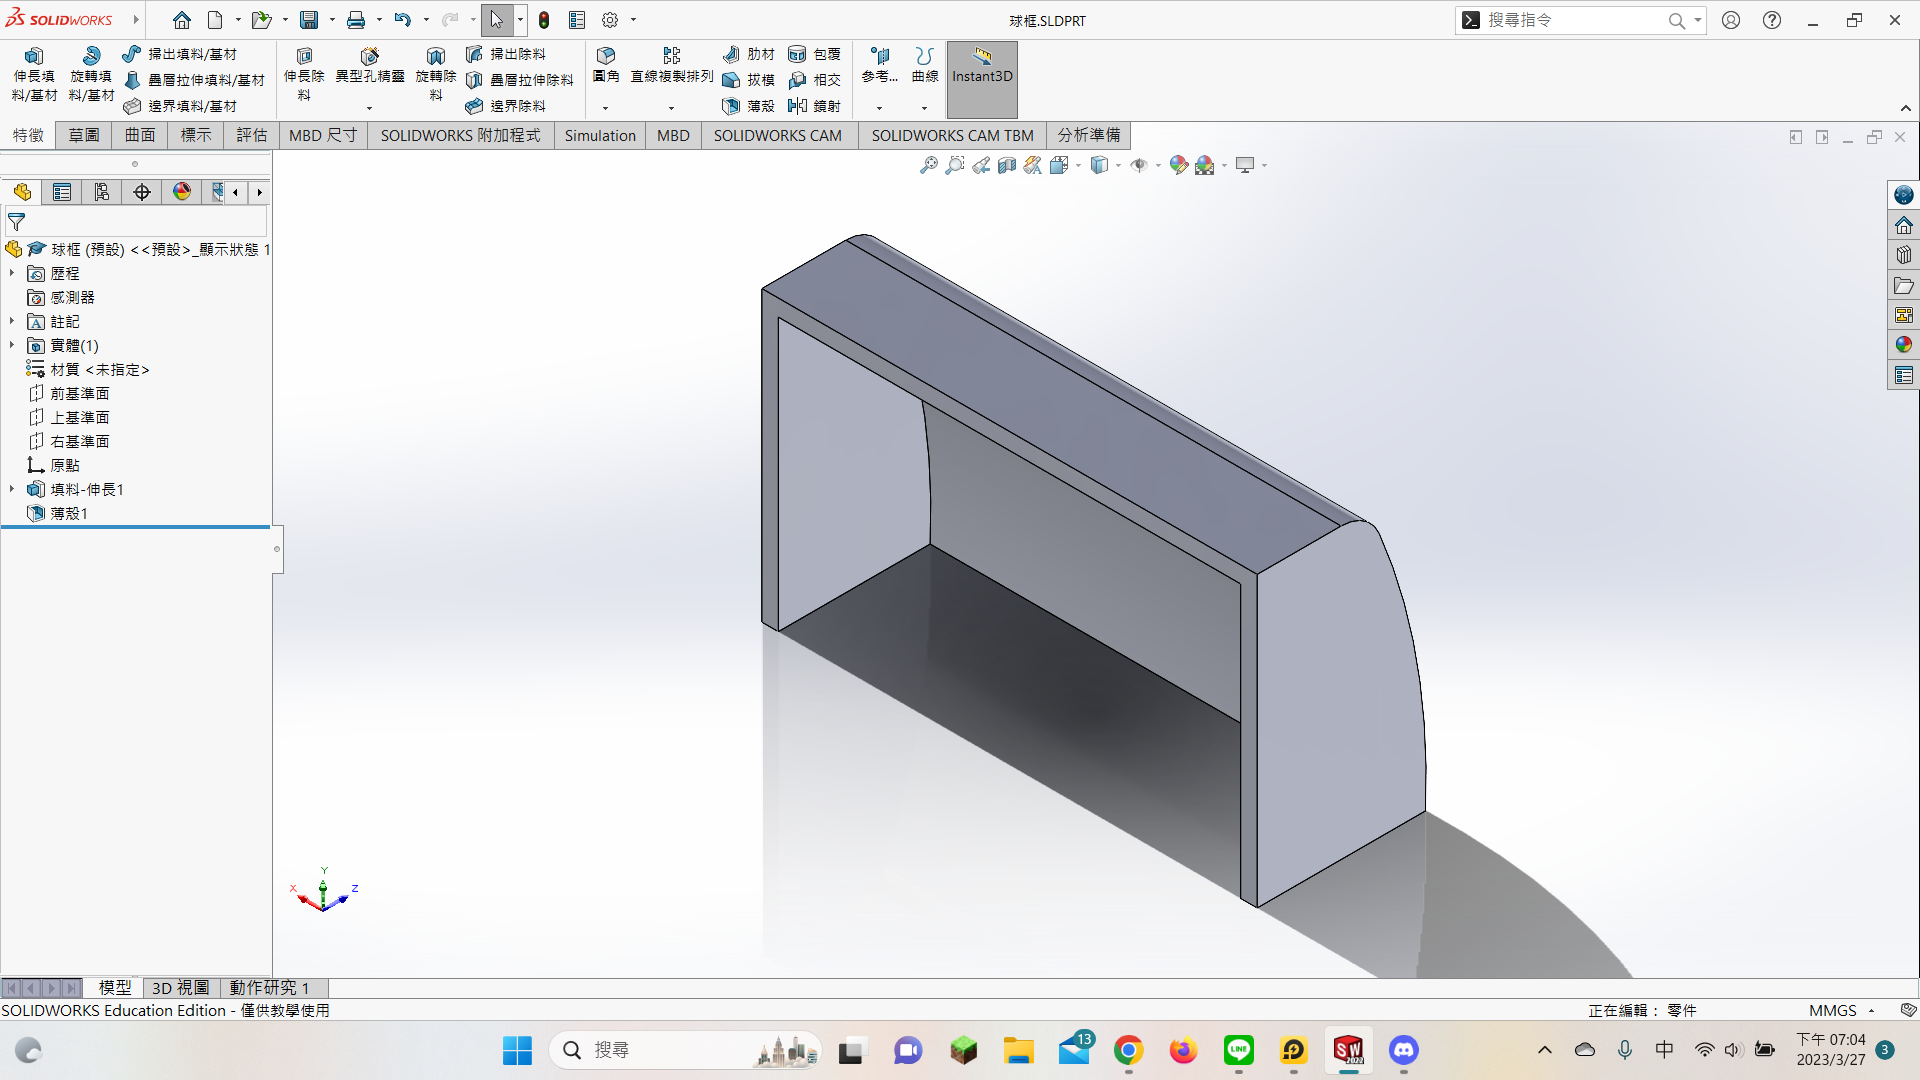
\includegraphics[angle=0,width=10cm]{2023-03-27}\\
\\2.這是lua腳本控制是bubbleRob前後左右sim.getObjectHandle這個函式在coppeliasim4.3.0版本被淘汰了但還是可以使用,但用sim.getObject會比較好在後面感測器腳本已做改善,這個程式是用上下左右控制bubbleRob空白鍵暫停開始。\
\begin{center}
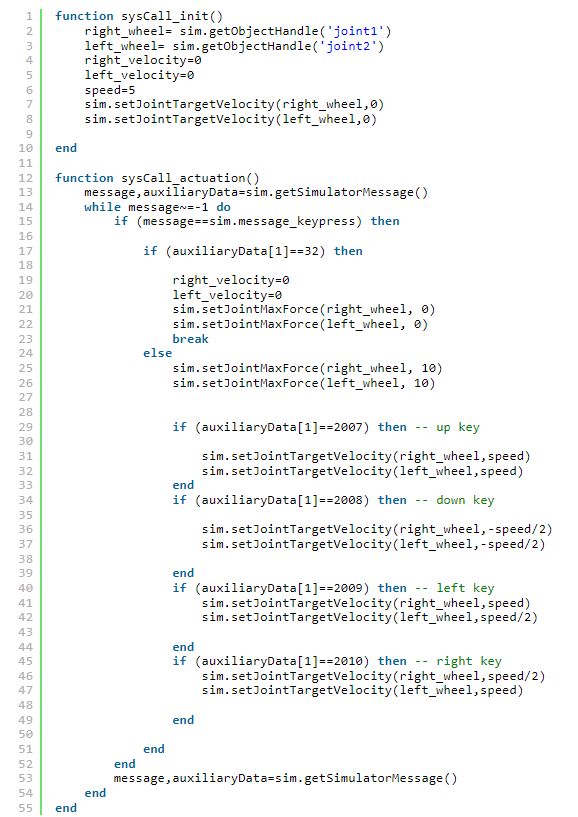
\includegraphics[angle=0,width=9cm]{螢幕擷取畫面 2023-04-14 221556}\\
\end{center}
 \newpage
3.加入球框感測器和記分板。\
\begin{center}
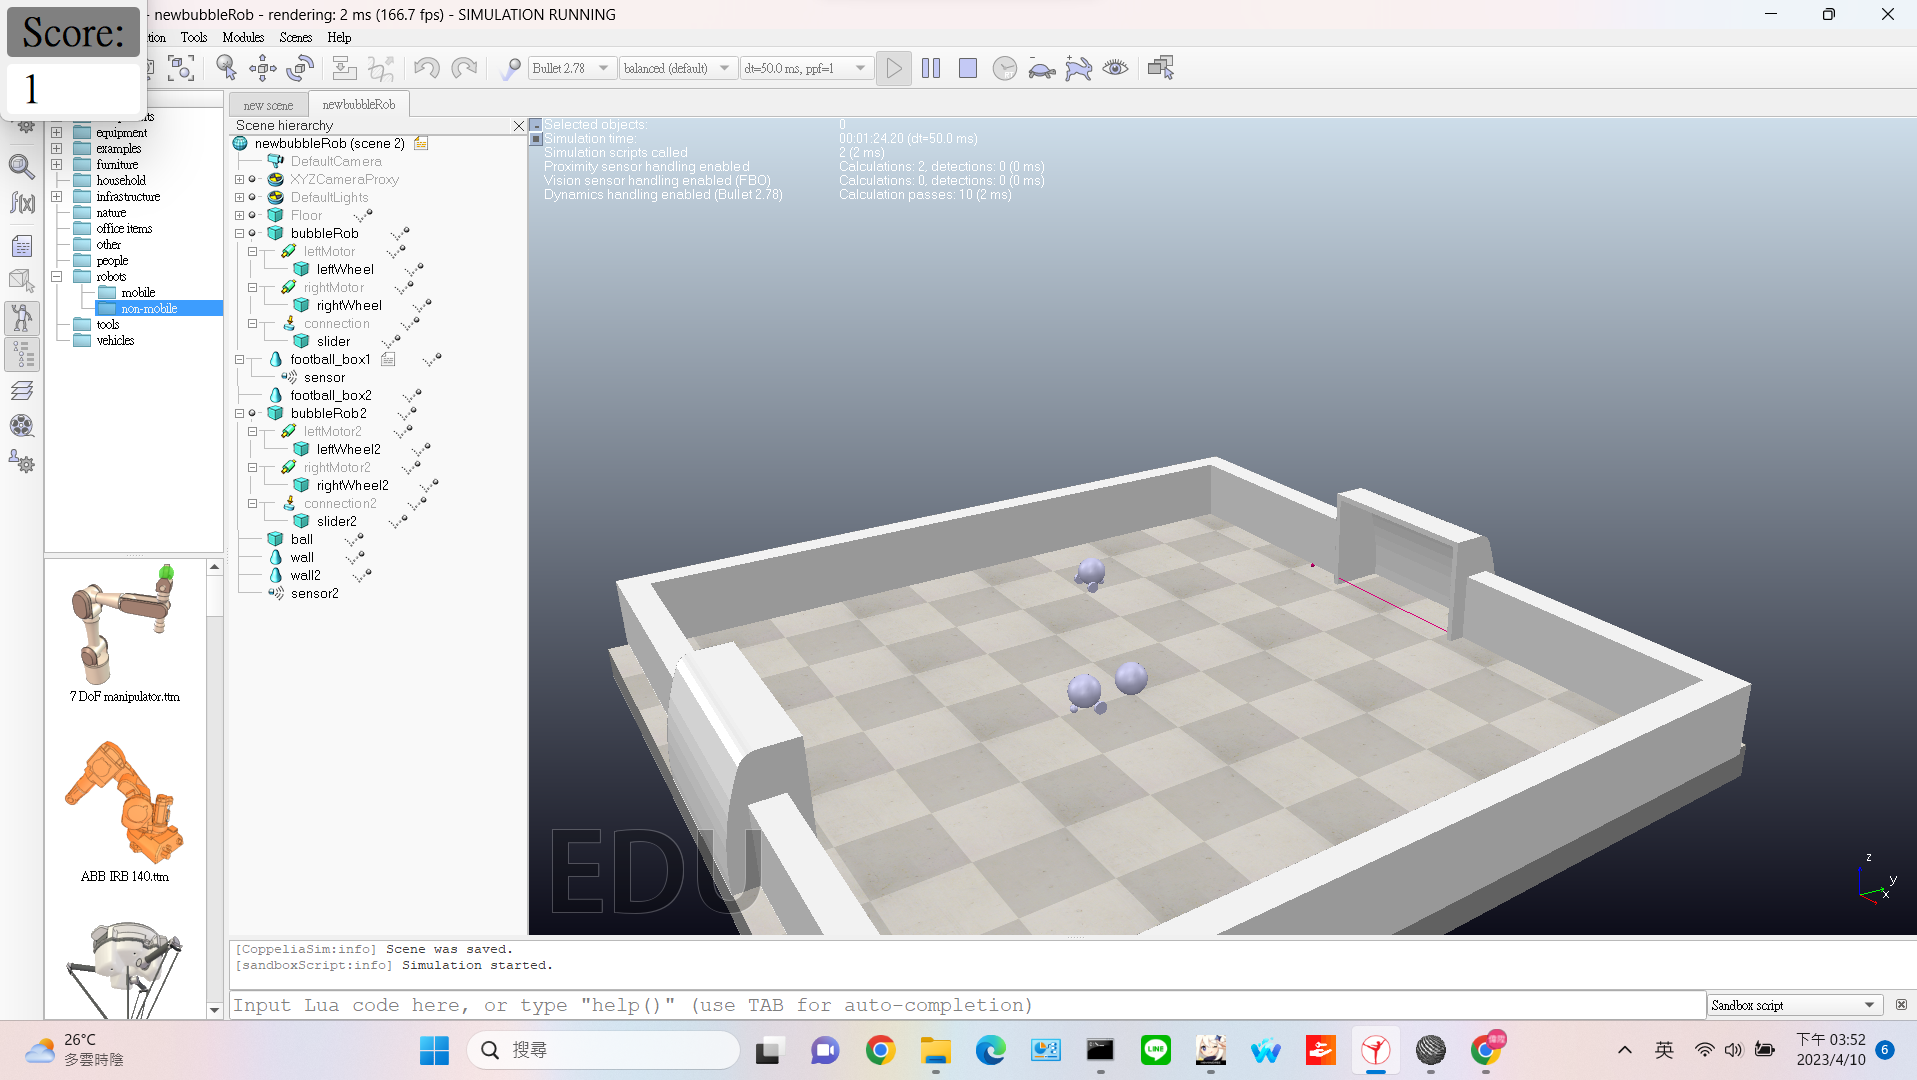
\includegraphics[angle=0,width=15cm]{football}
\end{center}

詳情可見\\
\href{https://mdecd2023.github.io/football-apj1/content/ag2.html}{https://mdecd2023.github.io/football-apj1/content/ag2.html}\\
\newpage
\begin{figure}[hbt!]
\chapter{環境設定}
\section{碰撞檢測}
\end{figure}
1.可探測(Detectable),可讓感測器感測到物體。在本遊戲中,球應該將Detectable打開,這樣才可以感測到進球,而bubbleRob機器人則要把Detectable關掉,不然機器人碰到感測器也會得分。\
\begin{center}
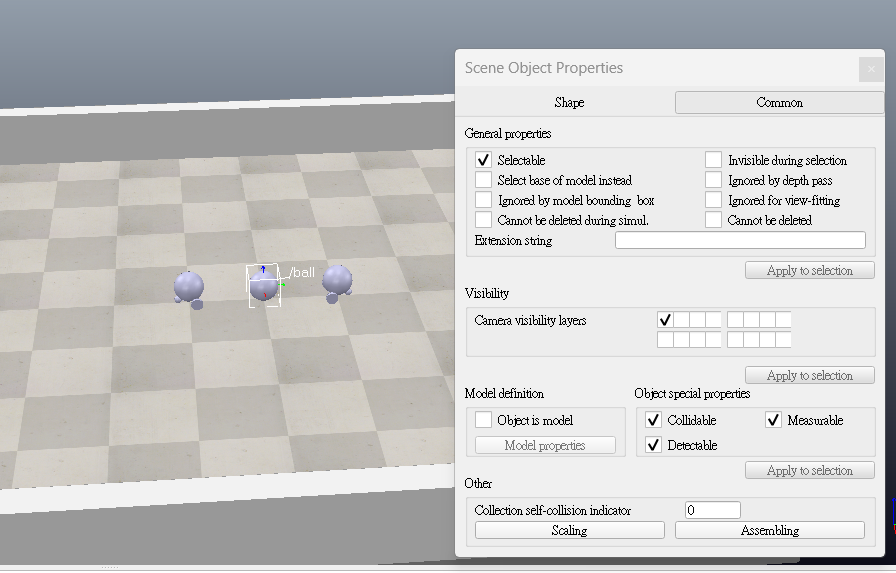
\includegraphics[angle=0,width=12cm]{48.1}\\
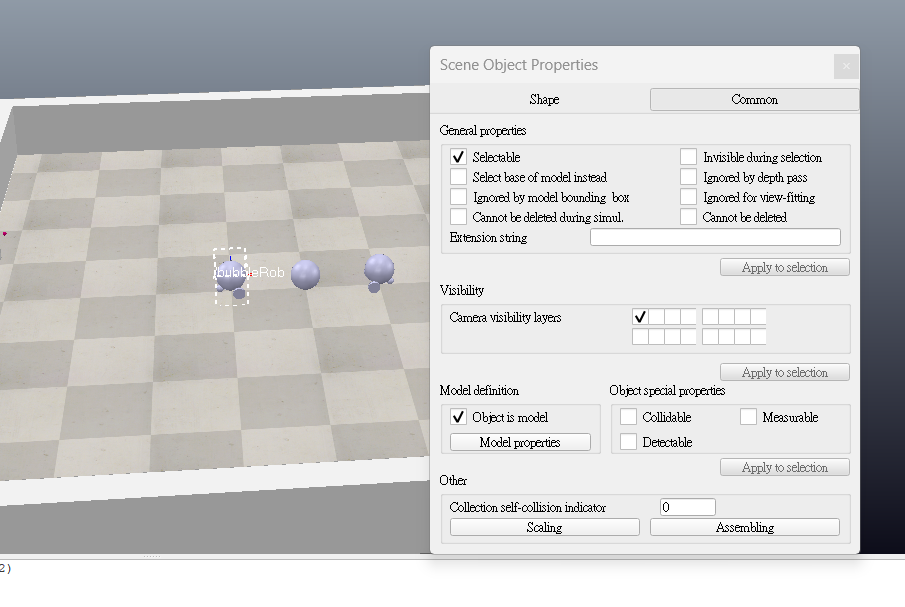
\includegraphics[angle=0,width=12cm]{48.2}
\end{center}
\newpage
2.在球框前加入射線感測器(Ray type),這樣球進框就一定會碰到感測器,射線感測器不能貼地不然感測不到。
\begin{center}
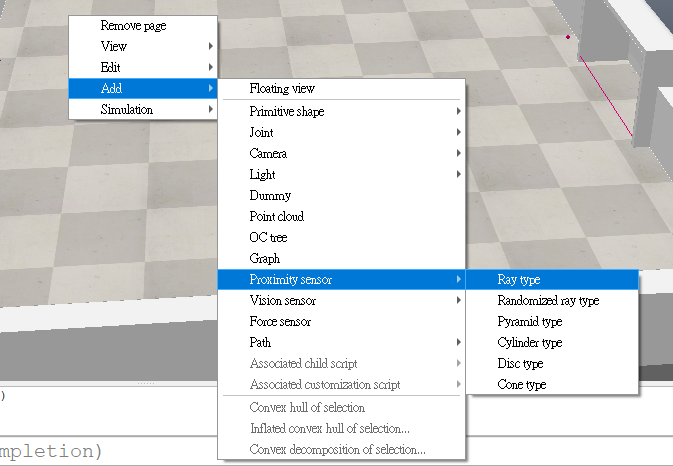
\includegraphics[angle=0,width=10cm]{48.5}
\end{center}

3.球框及圍牆的Body is respondable要打開不然球會穿過去,而Body is dynamic則要關上不然球框會亂動。
\begin{center}
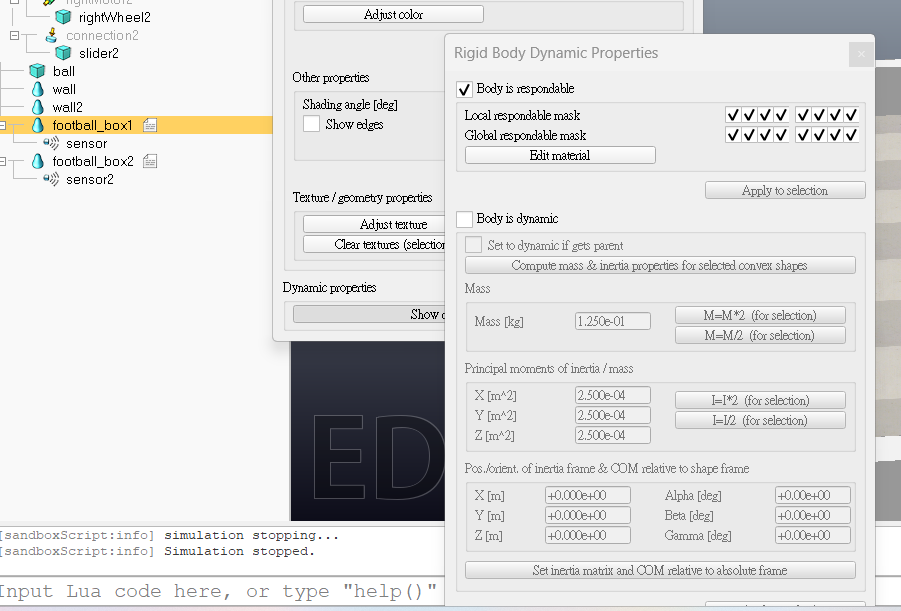
\includegraphics[angle=0,width=10cm]{48.3}
\end{center}

4.開啟Connectivity->Visualization,從http://127.0.0.1:23020/ 中可看見。
\begin{center}
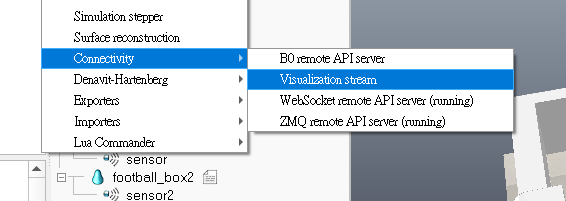
\includegraphics[angle=0,width=10cm]{4810}
\end{center}
\newpage
\begin{figure}[hbt!]
\chapter{程式}
\section{程式講解}
\end{figure}
1.先用xml製作記分板,然後用sim.getObjectPosition將bubbleRob、bubbleRob2和球的初始位置紀錄下來,然後用sim.getObjectOrientation將初始方向記錄下來。
\begin{center}
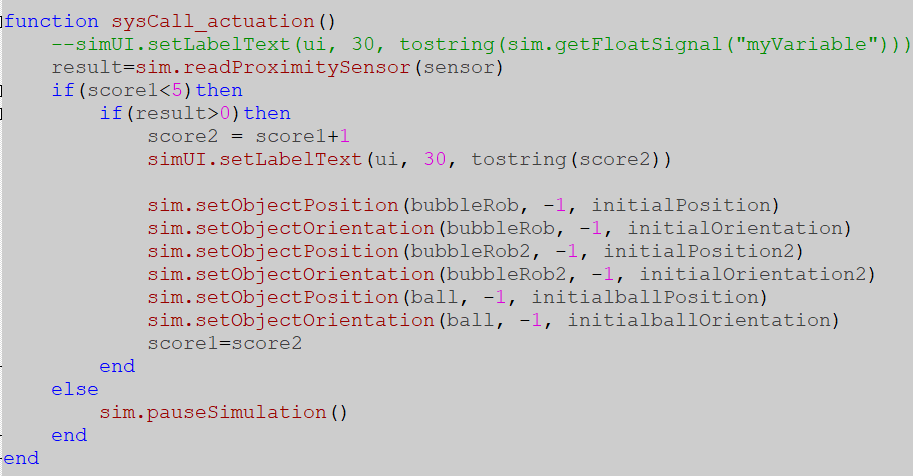
\includegraphics[angle=0,width=12cm]{48.4}
\end{center}

2.sim.readProximitySensor這個函數若傳感器未檢測到任何物體,返回值將是負數。如果傳感器與一個物體相交,返回值將是一個非負數的距離值,所以可以用if迴圈判斷函示返回值大於零去做加分跟回歸初始位置的動作
simUI.setLabelText(ui, 30, tostring(score2))這個函式則是將獲地的分數轉成string並輸入到id為30的text。
\begin{center}
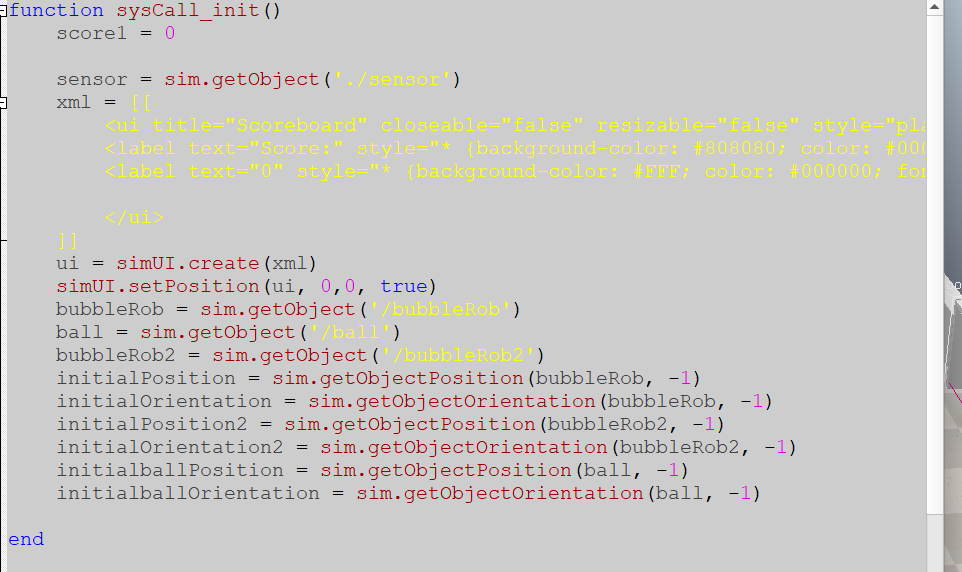
\includegraphics[angle=0,width=12cm]{48.6}
\end{center}
\newpage
3.這個程式要執行要先下載兩個東西pip install keyboard、pip install pyzmq cbor將這兩行打進cmd執行。
\begin{center}

\includegraphics[angle=0,width=15cm]{48.7}
\end{center}

4.這個程式要連線遠端電腦要將:\\
client=RemoteAPIClient('localhost', 23000)\\
中的localhost改成遠端電腦的ipv4位址並將遠端電腦的防火牆關掉,後面只要這個軸('/leftMotor')('/rightMotor')的名稱對應到coppeliasim就可以遠端控制。
\begin{center}
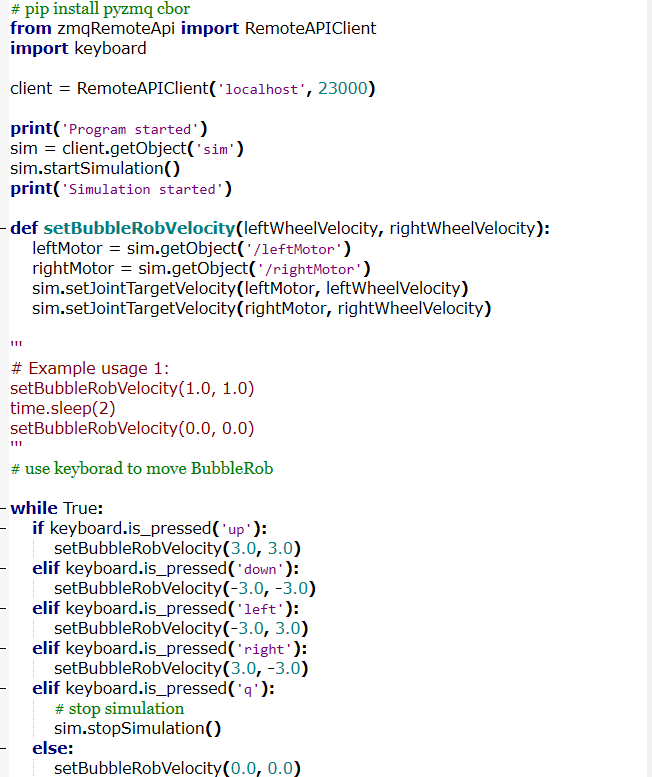
\includegraphics[angle=0,width=14cm]{48.8}
\end{center}
%=---------------------參考文獻----------------------=%
\addcontentsline{toc}{chapter}{參考文獻} %新增目錄名稱
\newpage
\renewcommand\bibname{參~考~文~獻}
\begin{thebibliography}{99}  % 參考文獻印出之編號最寬為兩個字母寬
\bibitem 1\href{https://www.coppeliarobotics.com/helpFiles/index.html}{https://www.coppeliarobotics.com/helpFiles/index.html}
\end{thebibliography}
%=---------------附錄-----------------=%
\addcontentsline{toc}{chapter}{附錄} %新增目錄名稱
\begin{appendix}
\renewcommand{\thesection}{\bf 附錄 \Alph{section}}%設定標題名稱
\begin{center}
\fontsize{20pt}{0em}\selectfont\bf 附錄
\end{center}
\section*{LaTeX}
LaTex 為一種程式語言,支援標準庫 (Standard Libraries) 和外部程式庫 (External Libraries),不過與一般程式語言不同的是,它可以直接表述 Tex 排版結構,類似於 PHP 之於 HTML 的概念。但是直接撰寫 LaTex 仍較複雜,因此可以藉由 Markdown 這種輕量的標註式語言先行完成文章,再交由 LaTex 排版。
此專題報告採用編輯軟體為LaTeX,綜合對比Word編輯方法,LaTeX較為精準正確、更改、製作公式等,以便符合規範、製作。
 \begin{table}[htbp] %htbp代表表格浮動位置
			\centering%表格居中
			\caption{文字編輯軟體比較表}%表:標題
			\large%字體大小
			\label{tab_文字編輯軟體比較表:scale}
			\begin{tabular}{|c|c|c|c|c|c|c|}
			\hline
			\diagbox[width=5em]& 相容性 & 直觀性 & 文件排版 & 數學公式 & 微調細部\\ 
			\hline
			LaTeX 		&$\surd$&		&$\surd$&$\surd$&$\surd$\\
			\hline
			Word	 	&		&$\surd$&		&		&$\surd$\\
			\hline
			
			\end{tabular}
		\end{table}	

\begin{itemize} 
\item 特點:
\end{itemize}
\begin{enumerate}
\item 相容性:以Word為例會有版本差異,使用較高版本編輯的文件可能無法以較低的版本開啟,且不同作業系統也有些許差異;相比LaTeX可以利用不同編譯器進行編譯,且為免費軟體也可移植至可攜系統內,可以搭配Github協同編譯。
\item 文件排版:許多規範都會要求使用特定版型,使用文字編譯環境較能準確符合規定之版型,且能夠大範圍的自定義排定所需格式,並能不受之後更改而整體格式變形。
\item 數學公式呈現:LaTex可以直接利用本身多元的模組套件加入、編輯數學公式,在數學推導過程能夠快速的輸入自己需要的內容即可。
\item 細部調整:在大型論文、報告中有多項文字、圖片、表格,需要調整細部時,要在好幾頁中找尋,而LaTeX可以分段章節進行編譯,再進行合併處理大章節。
\end{enumerate}
\begin{figure}[hbt!]
\begin{center}
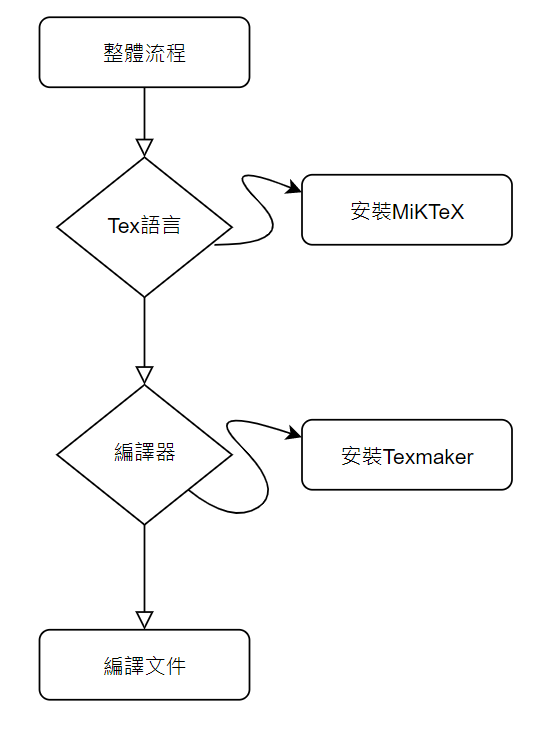
\includegraphics[width=10cm]{編譯流程}
\caption{\Large 編譯流程}
\label{fig.編譯流程}
\end{center}
\end{figure}
\end{appendix}
\section*{FFmpeg}
FFmpeg是一個開放原始碼的自由軟體,可以對音訊和視訊進行多種格式的錄影、轉檔、串流功能。在專題訓練過程中透過FFmpeg的視訊錄製的功能記錄對打影像來了解實際訓練狀況。
\newpage

%\newpage
%\begin{landscape}  %橫式環境
%\begin{center}
%\fontsize{0.001pt}{1pt}\selectfont .
%\vspace{70mm}
%\rotatebox[origin=cc]{90}{\LARGE 【14】}\rotatebox[origin=cc]%{180}{\LARGE 1-2-APP-8765} %旋轉
%\end{center}
%\end{landscape}
\end{document}
